\documentclass[a4paper,twocolumn]{article}

\usepackage{amsmath}
\usepackage{graphicx}
\usepackage{hyperref}
\usepackage{tabularx}
\usepackage{nth}

\title{Forensics analysis of USB device traces\\
\large Digital Forensics}

\author{
\begin{tabular}{>{\raggedleft}m{5cm}m{5cm}}
I. Duits & (1876171) \\
E. Geretto & (1869426) \\
G. Iadarola & (1879480) \\
\end{tabular}
}

\begin{document}
\maketitle

\abstract{The use of computers has increased exponentially in the last decade,
	so has cybercrime and the need for digital forensics. The use of Linux
	computers is growing, but there are just a few digital forensics tools
	that can scan a Linux image and support for Ext4 file system is poor on
	Windows. In this paper we will give an overview of Linux logging daemons
	and we will introduce a tool, USB Log Parser, which is able to retrieve
	information about USB devices from Linux log files, helping to cover the
	gap in compatibility of forensics tools with Linux. The tool covers most
	of the commonly used Linux distributions, like Ubuntu and Fedora,
	handling differences in logging systems.}

\section{Introduction}
\label{sec:intro}
Nowadays, our entire life is managed through electronic devices and the number
of connected users is going to grow in the future. Nevertheless, several
problems have to be faced in order to keep benefiting from the computing devices
revolution.

Everyone can get access and interact with PCs and smartphones and also criminals
are using them to perpetrate illegal activities. Indeed, the Digital Forensics
branch is becoming one of the most important sectors in the forensics and
investigation field. By inspecting and analysing computer systems, officers can
retrieve essential evidence to reconstruct criminal events.

Log files are one of the most important sources of information when trying to
understand how a certain state was produced on a given machine. They are
constructed recording a series of time stamped messages, generated by the
various components of the system, that, when considered as a whole, give a
complete overview of the operations in execution at a given moment.

Given the information they contain, log files are also one of the most important
sources of information during a forensics investigation since they allow to
trace possibly malicious activity through time. As a consequence, it is
essential to be able to retrieve and analyse them in the fastest way
possible.~\cite{finlayson1987log}

One of the main problems when analysing log files is that they tend to be huge
in terms of the number of messages collected in them. For this reason, forensics
investigators usually rely on tools that automatize the process of extraction
and parsing in order to extract immediately the relevant information.

One of the main problems in the retrieval of log files is that each operating
system, and sometimes each different version, uses a different log format. For
this reason, different tools are required in order to be able to analyse a
system efficiently.

The percentage of Windows desktop and laptop users is around 90\%~\cite{usagePC}
and the digital forensic tools available follow this line since most of them
runs on Windows only. For instance \emph{FTK Imager}, which is a useful tool
used by many investigators, only partially supports Ext4, which is a standard
format for Linux systems. By looking at the statistics, Linux users hold a 2\%
percent market share, but more than 66\% of internet servers runs a Linux
distribution and, taking into account only Web developers, 22\% of the
programmers work on Linux~\cite{usagePC}.

Unfortunately, Windows does not have native support for Linux file systems. The
open source community has responded to the challenge and created some excellent
software to solve this problem, like Ext2Read~\cite{ext2read}, but investigation
can be highly time sensitive and being able to recover automatically the
information needed from a system, without manual examination, can make a
difference.

In addition, since the source code for open source programs is available online,
it is really common for developers not to bother writing formal documentation.
In order to understand how a certain format is structured, it is common to be
forced to read blog posts or source code, instead of canonical documentation.
This tendency, unfortunately, is reflected also in the references of this
document.

This paper aims to contribute in filling these information gaps by presenting an
overview on Linux logging daemons and by introducing a tool, USB Log Parser,
which is able to retrieve information about USB devices. The tool was developed
by the authors as a forensic sound tool which can help digital forensic
investigators in extracting useful information about USB devices through the
examination of Linux log files.

USB devices can be used to transfer valuable data in cases of data theft or
possession of illegal material; knowledge about when a USB device was connected
can be really helpful in the investigation. As implied by the Locard's exchange
principle~\cite{locard2008locard}, every contact leaves a trace. These traces
are recoverable as reported, for instance, by several researches available in
the literature.~\cite{Tanushree12,Abhijeet14}

In Section~\ref{sec:lit}, this paper discusses how to access this information in
both Windows and Linux systems. The approach taken and the general structure of
the tool are instead described in Section~\ref{sec:contrib}. The tool was tested
on various images of Linux installations, the results for one of them are
presented in Section~\ref{sec:result}. The last section contains instead a short
summary of our conclusions.

\section{Log files and USB devices}
\label{sec:lit}

Given that different operating systems generate log files structured in a
different way and store them at different locations, the following subsections
will provide an overview of where the files are located and which tools can
be used to analyse them in Linux and Windows. Moreover, particular attention
will be given to the information relative to USB devices, since it is the main
focus of this study.

\subsection{Windows}\label{sec:litWindows}
In the newest iterations of Microsoft Windows, all the log files are stored by
default in a folder located at
\texttt{\%SystemRoot\%\textbackslash{}system32\textbackslash{}winevt\textbackslash{}Logs}.
These files can be opened with a tool called \emph{Event Viewer} in order to
examine their content. This tool, however, allows only for simple automatic
analysis, as a general keyword search, but it does not automatically extract
the most relevant information stored.

From a forensics investigator perspective, the use of Event Viewer implies a
tedious and error prone manual analysis that is surely not desirable. For this
reason, other tools have been developed that allow the extraction and analysis
of log files from system images in an automatic fashion, so that the
investigator just needs to observe the relevant data and connect them to the
evidence already collected.

These tools are time saving and, most importantly, the analysis of the evidence
can be considered forensically sound. Indeed, in order to avoid damaging or
contaminating the evidence collected, the system analysed should always be
imaged and the image should be hashed in order to allow for a subsequent
verification of the investigative process. These tools allow for the analysis of
these images directly and guarantee the absence of contamination during the
process.~\cite{murphey2007automated}

The open source tool that is most commonly used for this purpose is called
\emph{Autopsy}, developed by \emph{SleuthKit}~\cite{sleuthkit}; between other
things, it also analyses the system logs and extracts a list of all the USB
devices that were attached to the machine according to the information in the
files. This allows an investigator to retrieve important information, as the
serial number of the device or the time of insertion and deletion. This
information is important, for example, to track USB sticks across different
machines.~\cite{deb2015usb}

\subsection{Linux}
Regarding the Linux operating system, the kernel has an internal log on which
every module can write, including the USB drivers. This log, called internal
ring buffer, is not directly stored in persistent memory; this task is demanded
to other services that also collect logs from other sources, as the \emph{X11}
display server, and construct a general system log.

Unfortunately, different distributions use different log-handling daemons and
even different versions of the same daemon may store the log files in
different locations. The most common ones are the \emph{syslog} daemon, which
stores the log in the \texttt{/var/log/syslog} file in plaintext, and the
\emph{journald} daemon, part of the systemd project, which stores the files in
the \texttt{/var/log/journal/} directory in binary format. There are also other
interesting combinations that include collecting the data using journald and
then store them in a syslog compatible format, as Ubuntu and derivatives
do.~\cite{poettering2012journal}

All the USB related information flows from the kernel ring buffer to the log
daemon and gets stored in one of these locations. Given the variety of locations
and daemons that are currently being used, to the best of our knowledge, there
is no automated tool that is capable of extracting automatically, from a disk
image, information about USB devices; currently, the only option is manual
analysis.

\section{USB device tracking on Linux}
\label{sec:contrib}
Given the absence of a forensics tool that is capable of analysing images taken
on Linux systems in order to retrieve USB device information, it was decided to
implement one in Python leveraging several libraries already available.

Since the data that needs to be retrieved can be found in two forms, namely
syslog text files or journald binary log files, it was decided to implement a
tool capable of distinguishing between the two and parse both file formats.

In Subsection~\ref{sec:prems} all the dependencies and compatibility
considerations will be listed, explaining the reasons behind the choice of the
supported distributions. Subsection~\ref{sec:images} will instead be used to
describe the procedure followed for the creation of the images used in the
study. Finally, Subsection~\ref{sec:tool} will describe the general structure of
the tool and the reflections made while constructing it. Given that the tool is
opern source, the code is available online.~\cite{ourtool}

\subsection{Dependencies and compatibility}
\label{sec:prems}
In the development of our tool, we used two main libraries that need
to be installed on the machine performing the analysis:
\texttt{imagemounter} and \texttt{python-systemd}. Both the libraries were used
in their Python 3 version.

Regarding \texttt{imagemounter}, it is simply a wrapper for
SleuthKit~\cite{sleuthkit}, a set of tools on which Autopsy, mentioned before,
is also based.  This library offers APIs that make mounting an EnCase image from
inside a Python script quite easy, allowing then the program to explore the
directories required for the analysis.

The \texttt{python-systemd} library is instead a Python wrapper for the C APIs
that allow the interaction with the journald log daemon. The use of this library
was necessary in order to parse the binary format in which the logs are stored
and extract the relevant information. The positive thing about the use of this
module is that it grants access to all the information related to the production
of the log format, for example the kernel subsystem that actually created a
certain message.

Regarding instead the supported distributions, the choice of supporting Ubuntu
was quite obvious. This distribution indeed, apart from having a large market
share by itself, is also the base for many others, as Linux Mint, all the Ubuntu
spins and Elementary OS to name a few. Taking all these distributions into
consideration, a good percentage of the Linux desktop users is covered.

Regarding the choice related to how the system logs are stored, the Ubuntu
developers made the choice of exploiting the new functionalities introduced by
systemd, but to avoid storing the logs in binary format. As a consequence,
Ubuntu uses journald to collect the logs but then dumps them in a syslog
compatible log, as already described before and in the
literature.~\cite{patil2016digital} For this reason, the support of Ubuntu
required the writing of a parser for that particular format.

Given that syslog compatible logs were covered, Fedora was chosen as the second
distribution to be supported. This choice was done because it is one of the main
distributions that, as opposed to Ubuntu, use the journald binary format.

A third distribution that was evaluated for the analysis was OpenSUSE
considering, again, its market share and the similarity to its commercial
counterpart, SUSE Linux Enterprise. Unfortunately, after completing the imaging
process, we realized that the file system used for the root partition in
OpenSUSE, the new BtrFS introduced some years ago, is still not supported by
\texttt{imagemounter}, since it is not commonly used. For this reason, we had to
exclude it from the analysis.

As far as the compatibility of the tool is concerned, it is restricted to the
same compatibility of the libraries \texttt{python-systemd} and
\texttt{imagemounter}. On the positive side, since the tool is based on these two
libraries, its compatibility will improve when these libraries will extend
the support for different systems.

Regarding the versions of the distributions used, we employed Fedora 25 and
Ubuntu 17.04, the latest versions available at the moment of writing.

\subsection{Creation of the images}
\label{sec:images}
The machine used to collect the images was a HP ProBook 6570b with UEFI
support, on which every distribution was installed in sequence. For every
image, a similar iteration was followed:
\begin{itemize}
\item Installation with default settings.
\item Update to the packets available on the \nth{29} of May 2017.
\item Installation of all the missing drivers, in particular the WiFi one.
\item Insertion and extraction of one USB stick 2.0, one USB stick 3.0 and a USB
	mouse.
\item Reboot in a live environment.
\item Creation of a raw image of the root partition.
\item Conversion of the image in EnCase format using FTK Imager.
\end{itemize}
It is relevant to point out that the hash of the images was checked across the
whole process in order to prevent any kind of corruption.

\subsection{The tool}
\label{sec:tool}
Once in possession of the images, it is possible to feed them to the tool in
order to receive as output a table containing various information related to all
the USB devices that were connected to the systems, according to the system
logs.

Under the hood, the tool exploits the capabilities of the \texttt{imagemounter}
library to try to mount every volume contained in the EnCase image provided and
checks if it is a root Linux file system containing the standard log directory.
If this is the case, the tool determines then which one between syslog and
journald was used to collect the logs and then starts the parsing process using
the appropriate submodule.

It is important to note that, if several Linux installations are present on the
same system, as in a dual boot context, the tool will correctly detect both
installations and present the results related to both systems. All other
partitions will simply be ignored.

After the individuation of the log files, according to the type of log, the
file is feed to a different submodule. The one processing syslog files takes
care of filtering, one by one, the lines from the full system log and extracts
only those that have been generated by the USB subsystem, while the second
leverages the \texttt{python-systemd} library in order to parse the binary file
and achieve the same result through filters on the fields in the binary
entries.

Once all the messages generated by the USB subsystem are obtained, the tool
starts looking for fixed string patterns in order to extract information from
lines about USB devices. Some patterns were created to localize lines
which store information about time of connection, both in and out, and
regarding product name, manufacturer and serial number.

The tool analyses all the messages generated by the USB subsystem and, when a
pattern matches one, the line is parsed and the information retrieved. The new
data is then saved inside an object which stores all the information found for
the same USB device. Finally, all the information is printed grouped by USB
device.

Given that the tool is based on the libraries \texttt{imagemounter} and
\texttt{python-systemd}, the forensic soundness of its operations is implied by
the operations of these libraries. The other tools that use these libraries are
well-known forensic tools and they are considered reliable by the forensics
community. For instance, \texttt{imagemounter} is a wrapper for SleuthKit, used
by Autopsy as well~\cite{sleuthkit}. Moreover, the tool does not work on the
original data but just on copies of them, since it handles images of Linux
distribution in EnCase format, which preserve integrity. Finally, all the code
is open source and everyone can verify the correctness of every operation.

\section{Results}
\label{sec:result}
As described before, the validation of the tool was made using several EnCase
images; this section will analyse the output generated by the one containing
Ubuntu 17.04.

The operations listed in Section~\ref{sec:images} were operated on the machine
while Ubuntu was installed. As a consequence, the tool is expected to recover
the information related to two USB sticks, a 2.0 and a 3.0 one, and a USB mouse.
The output of the execution, which took less then a two seconds, is presented in
Figure~\ref{fig:restool}.

\begin{figure*}[t]
\centering
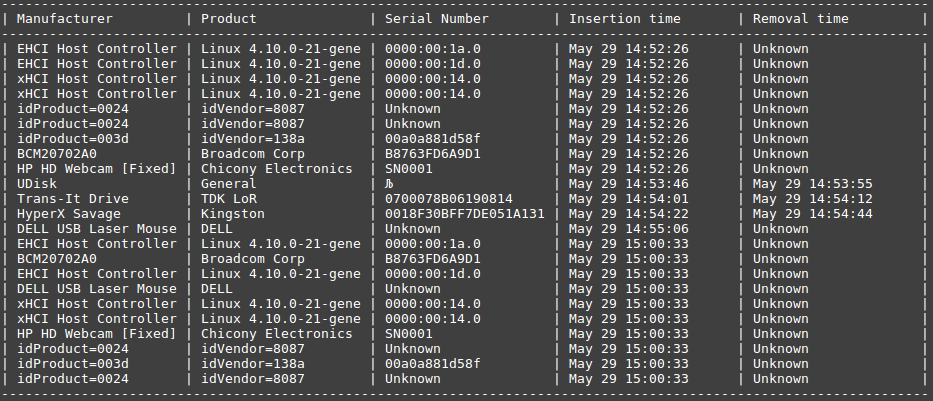
\includegraphics[width=\textwidth]{images/ubu_res.PNG}
\caption{Output of the tool after the analysis of the Ubuntu image.}
\label{fig:restool}
\end{figure*}

Lines 10--12 of the table created by the tool show the information related to
the USB sticks listed before. The tool was also able to extract the serial
number and the insertion and removal time for these devices. The other lines are
related to the internal USB devices, like webcam and USB hubs. The mouse is
instead listed at lines 11 and 15.

The main reason why the removal time is not present for most of the devices is
that no disconnection message is inserted in the log if the computer is turned
off and the device is disconnected right after.

The steps performed in this section are replicable by everyone since the tool is
available online.~\cite{ourtool}

\section{Conclusion}
\label{sec:concl}
It is a matter of fact that Windows does not have native support for Linux file
systems. Since the most used forensic tools run on Windows, analysing Linux
systems is harder than Windows ones.

Nevertheless, for the sake of completeness, the investigators cannot assume that
the criminals will use Windows only. As already discussed in
Section~\ref{sec:intro}, Linux systems hold a relevant part of the market share
when considering skilled users. Because of that, it is really important to
develop software that handles all the possible distributions and file systems in
order to produce precise and complete investigations. On this assumptions, our
tool can contribute in analysing USB device traces on Linux systems.

Our tool is able to retrieve logs quickly, as demonstrated in
Section~\ref{sec:result}. By extracting and parsing only a restricted set of
files, it reports the USB traces immediately. Obviously, it cannot produce a
complete analysis of the images but it will not waste time in deep analysis when
it is not required. Indeed, when USB devices are involved during an
investigation, just demonstrating the connection to a victim machine can be
enough to prove the criminal act. As far as the authors know, there are no tools
which are able to analyse EnCase images of a Linux operating system and retrieve
automatically information related to USB devices; the only technique available
is to check manually the log files, a really time consuming operation.

Moreover, the analysis produced by the tool is forensically sound, because it
does not compromise the integrity of the images; in fact, the elaboration is
based on EnCase images, which embed a hash of the data that is verified before
every analysis. Moreover, the libraries the tool relies on are well-known in the
forensics community and ensure the correctness of the results.

In conclusion, this paper presented an overview on log files across different
operating systems in order to compare logging methods on different platforms.
After that, it presented a tool which aims to contribute in the forensic field
by simplifying the analysis of USB device logs on Linux systems.

\bibliographystyle{plain}
\bibliography{sample}

\end{document}
